\chapter{Bất định, định lý Ehrenfest và giới hạn cổ điển}

\section{Điểm còn dang dở trong Hamiltonian tuyến tính}

Mô hình
\begin{equation}
H=cP
\label{eq:l10-linear-hamiltonian}
\end{equation}
đã hữu ích vì các gói sóng của nó tịnh tiến mà không đổi dạng. Nó cũng mang theo một cảnh báo nghiêm trọng. Động lượng có thể dương hoặc âm, nên cùng một công thức gán năng lượng dương cho một sóng phẳng và năng lượng âm cho sóng kia:
\begin{equation}
\psi_p(x)=e^{ipx/\hbar},
\qquad
E(p)=cp.
\end{equation}
Nếu có thể có tùy ý nhiều hạt vật lý chiếm các trạng thái năng lượng âm, thì không gian trống sẽ không phải là trạng thái có năng lượng thấp nhất. Nó có thể tạo ra các lượng tử năng lượng dương đồng thời đưa năng lượng âm bù trừ vào các hạt mới, bảo toàn tổng năng lượng nhưng hạ thấp chân không mà không có cận.

\begin{classroomqa}
\audiencequestion{Vì sao một nhánh năng lượng âm lại không chỉ là một cách chọn mốc không hơi kỳ lạ cho năng lượng?}
\lecturerresponse{Một phép dời cộng chung lên mọi mức năng lượng thì vô hại. Một phổ không bị chặn thì khác. Nếu các trạng thái có năng lượng ngày càng thấp vẫn có thể bị chiếm, trong khi các hạt năng lượng dương mang phần cân bằng đi, thì sẽ không có trạng thái cơ bản ổn định. Tính ổn định đòi hỏi một cận dưới so với chân không.}
\end{classroomqa}

\begin{figure}[htbp]
\centering
\includegraphics[width=0.88\textwidth]{lecture_10_figure_01.png}
\caption{Hamiltonian tuyến tính và các hàm riêng sóng phẳng của nó làm lộ ra nhánh năng lượng âm khi \(p<0\).}
\lectureframe{00:04:35}
\end{figure}

Câu trả lời lịch sử của Dirac có tác dụng đối với fermion. Fermion tuân theo nguyên lý loại trừ: không có hai fermion đồng nhất nào có thể chiếm cùng một trạng thái một hạt. Hãy hình dung lấp đầy mọi trạng thái năng lượng âm. Một khi tất cả chúng đã bị chiếm, nguyên lý loại trừ ngăn không cho một fermion khác rơi vào khu vực đó. Một chỗ trống trong tập đã lấp đầy ấy hành xử như một phản hạt.

Lập luận này không cứu vãn được các boson năng lượng âm. Bất kỳ số lượng boson nào cũng có thể chiếm một trạng thái, nên một mode boson năng lượng âm có thể bị lấp đầy không giới hạn. Bức tranh biển đầy cũ tốt nhất nên được xem như con đường lịch sử dẫn tới phản hạt; lý thuyết trường lượng tử hiện đại tổ chức hạt và phản hạt mà không coi chân không vật lý là một biển electron năng lượng âm quan sát được theo nghĩa đen. Điểm cần ở đây hẹp hơn: Hamiltonian đồ chơi này không phải là một lý thuyết hạt ổn định hoàn chỉnh.

Như một mô hình biếm họa một chiều của một hạt fermion chuyển động với tốc độ cố định, mô hình này gợi đến bài toán neutrino mà các ý tưởng của Dirac từng có liên quan. Nó không thể dùng làm một lý thuyết photon: photon là boson, và nguyên lý loại trừ không thể lấp đầy rồi chặn các trạng thái năng lượng âm của chúng.

\begin{classroomqa}
\audiencequestion{Vì sao nguyên lý loại trừ có thể ổn định hóa cấu trúc fermion nhưng không thể làm vậy cho cấu trúc boson?}
\lecturerresponse{Một trạng thái fermion có thể được lấp đầy một lần rồi bị chặn. Một trạng thái boson không có trần số chiếm như vậy, nên một mode boson năng lượng âm vẫn sẽ cho phép năng lượng giảm xuống mà không có cận.}
\end{classroomqa}

\paragraph{Tình hình hiện tại của học phần.}
Trong học kỳ này, phần lớn nền tảng của cơ học lượng tử và một số hệ được cố ý chọn sao cho đơn giản đã được phát triển, nhưng ứng dụng thì rất ít. Đặc biệt, vẫn chưa đi tới ngay cả dao động tử điều hòa. Sự thiếu vắng ấy đánh dấu một ranh giới hơn là một kết thúc: tiếp theo là thuyết tương đối và lý thuyết trường, sau đó phải quay lại cơ học lượng tử để nghiên cứu dao động tử và các cấu trúc khác xây trên nó. Mối quan tâm bền bỉ đối với thảo luận trước đó về vướng víu lượng tử cũng cho thấy vì sao con đường đi qua phần nền tảng là đáng giá.

Với góc nhìn đó, điểm còn dang dở được khép lại. Công việc chính là hàm sóng, độ bất định, và mối quan hệ giữa sự tiến hóa lượng tử với cơ học cổ điển. Mục tiêu không phải là phương trình tiến hóa tổng quát nhất có thể, mà là phương trình đặc biệt trong không gian vị trí do Schr\"odinger viết ra ban đầu.

\section{Hàm sóng và các tọa độ giao hoán đầy đủ}

Đối với một hạt trên một đường thẳng, hàm sóng trong không gian vị trí là
\begin{equation}
\psi(x)=\braket{x}{\psi},
\end{equation}
đó là biên độ để tìm thấy hạt gần \(x\). Hàm sóng trong không gian xung lượng là
\begin{equation}
\widetilde{\psi}(p)=\braket{p}{\psi}.
\end{equation}
Chúng mô tả cùng một trạng thái trừu tượng trong các cơ sở khác nhau và liên hệ với nhau bằng một phép biến đổi Fourier:
\begin{align}
\psi(x)
&=
\int_{-\infty}^{\infty}
\frac{dp}{\sqrt{2\pi\hbar}}\,
\widetilde{\psi}(p)e^{ipx/\hbar},
\label{eq:l10-fourier-forward}\\
\widetilde{\psi}(p)
&=
\int_{-\infty}^{\infty}
\frac{dx}{\sqrt{2\pi\hbar}}\,
\psi(x)e^{-ipx/\hbar}.
\label{eq:l10-fourier-inverse}
\end{align}

\begin{figure}[htbp]
\centering
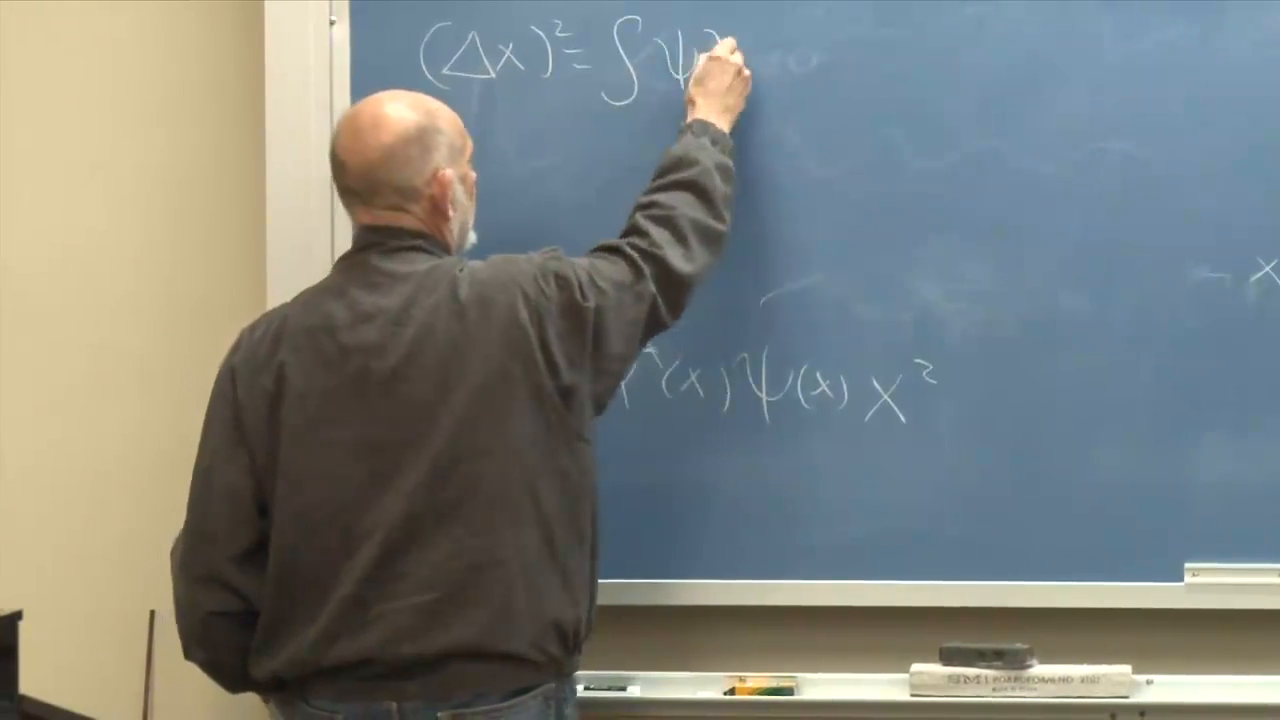
\includegraphics[width=0.88\textwidth]{lecture_10_figure_02.png}
\caption{Các hàm sóng theo vị trí và theo xung lượng là các hình chiếu của cùng một trạng thái lên hai cơ sở liên tục khác nhau.}
\lectureframe{00:09:05}
\end{figure}

Trong hai chiều không gian, \(X\) và \(Y\) giao hoán, nên một cơ sở riêng chung có thể được gắn nhãn bằng cả hai tọa độ và hàm sóng trở thành \(\psi(x,y)\). Tính giao hoán đó không bị ép buộc chỉ bởi riêng các tiên đề trừu tượng; nó là một phần của mô tả lượng tử đã thành công về mặt thực nghiệm của không gian thông thường. Đối với \(N\) hạt trong ba chiều,
\begin{equation}
\psi(\mathbf{x}_1,\ldots,\mathbf{x}_N)
\end{equation}
là một hàm trên không gian cấu hình, chứ không phải một sóng ba chiều riêng biệt gắn độc lập với từng hạt. Vì thế, một hệ vĩ mô có thể đòi hỏi một số lượng tọa độ khổng lồ.

\begin{classroomqa}
\audiencequestion{Việc các tọa độ không gian khác nhau giao hoán có tự động suy ra từ cơ học lượng tử hay không?}
\lecturerresponse{Không. Khung trừu tượng cho phép nhiều đại số các đại lượng quan sát. Việc các thành phần vị trí Descartes khác nhau giao hoán là một sự kiện cấu trúc mang tính thực nghiệm của cơ học lượng tử cho các hạt trong không gian thông thường.}
\end{classroomqa}

Ta có thể biến đổi Fourier mọi tọa độ để thu được một hàm sóng của tất cả các xung lượng, hoặc chỉ biến đổi những biến được chọn. Các biểu diễn hỗn hợp là hợp lệ vì một biểu diễn là sự lựa chọn cơ sở, chứ không phải sự thay đổi trạng thái vật lý.

\section{Độ bất định đo điều gì}

Dạng sơ khai nhất của nguyên lý bất định suy ra ngay từ cặp Fourier. Một trạng thái có xung lượng xác định là một sóng phẳng có môđun không đổi và không định xứ trong vị trí. Một trạng thái định xứ sắc trong vị trí đòi hỏi nhiều thành phần xung lượng. Tổng quát hơn, khi thu hẹp một thành viên của một cặp Fourier thì thành viên kia bị nới rộng.

\begin{figure}[htbp]
\centering
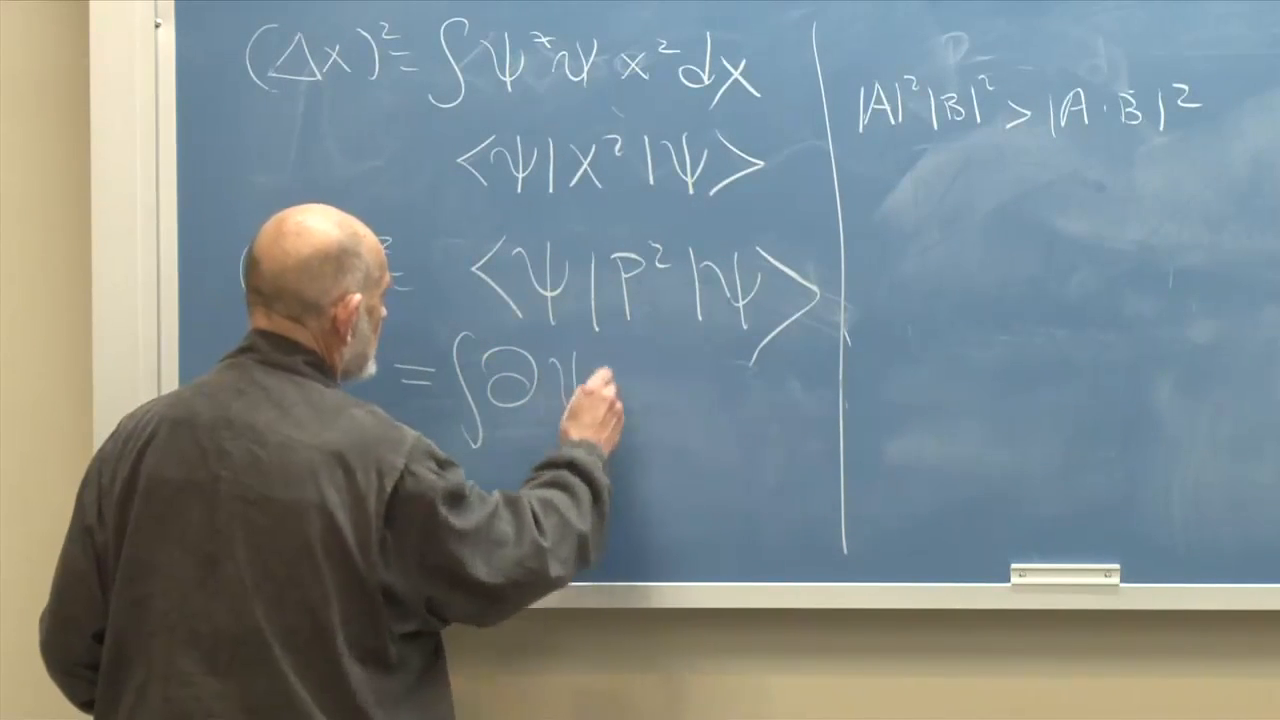
\includegraphics[width=0.88\textwidth]{lecture_10_figure_03.png}
\caption{Một phân bố vị trí định xứ đòi hỏi một chồng chập rộng các sóng phẳng trong biểu diễn xung lượng đối ngẫu.}
\lectureframe{00:14:45}
\end{figure}

Để phát biểu đó trở nên định lượng, hãy bắt đầu với một đại lượng quan sát tổng quát \(Q\). Giá trị kỳ vọng của nó trong một trạng thái đã chuẩn hóa là
\begin{equation}
\expect{Q}=\bra{\psi}Q\ket{\psi}.
\end{equation}
Phương sai là
\begin{equation}
(\Delta Q)^2
=
\expect{\bigl(Q-\expect{Q}\bigr)^2}
=
\expect{Q^2}-\expect{Q}^2.
\label{eq:l10-general-variance}
\end{equation}
Độ bất định \(\Delta Q\) là căn bậc hai dương của phương sai này.

Đối với vị trí, trước hết có thể dời gốc tọa độ sao cho \(\expect{X}=0\). Khi đó
\begin{equation}
(\Delta x)^2
=
\expect{X^2}
=
\int_{-\infty}^{\infty}
dx\,|\psi(x)|^2x^2.
\label{eq:l10-position-variance}
\end{equation}
Các đóng góp dương và âm triệt tiêu trong \(\expect{X}\), nhưng chúng cộng lại trong \(\expect{X^2}\). Vì vậy, một phân bố xác suất rộng hơn sẽ có phương sai lớn hơn.

\begin{figure}[htbp]
\centering
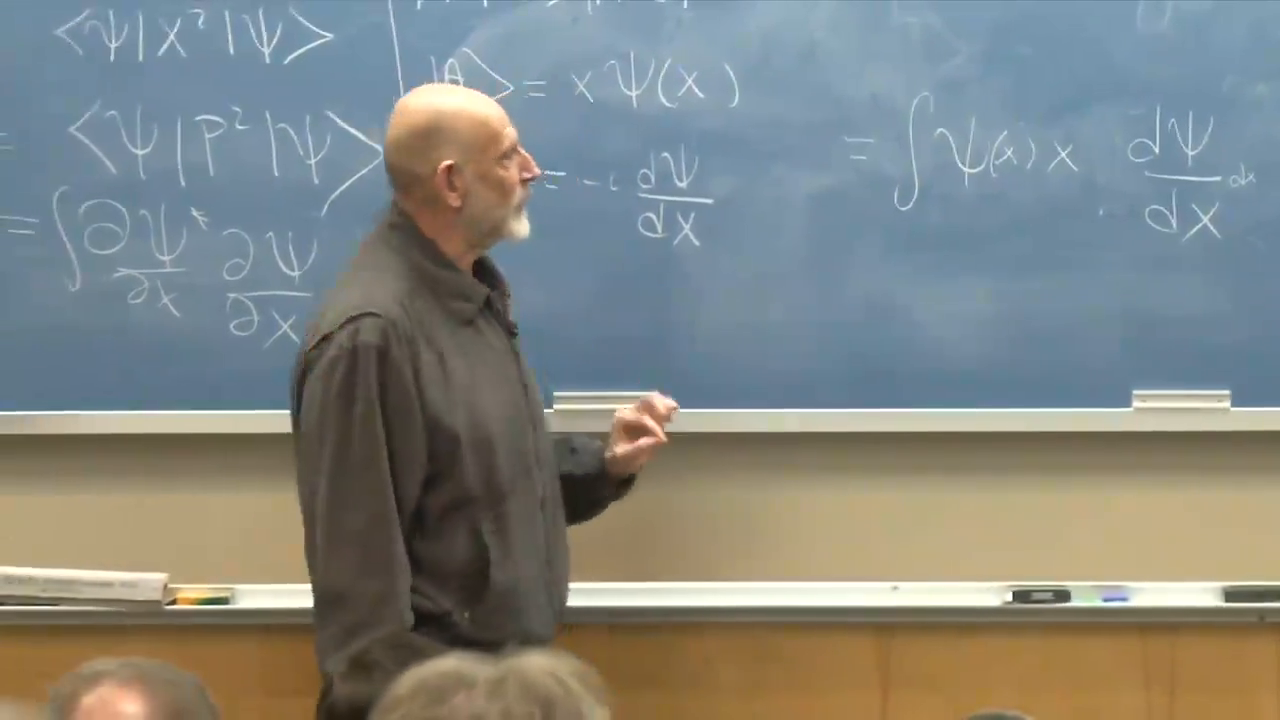
\includegraphics[width=0.88\textwidth]{lecture_10_figure_04.png}
\caption{Khi giá trị trung bình được dời về không, phương sai vị trí là tích phân có trọng số xác suất của \(x^2\).}
\lectureframe{00:20:50}
\end{figure}

Sự phân biệt giữa \(\expect{X^2}\) và \(\expect{X}^2\) là thiết yếu. Một phân bố đối xứng quanh không có \(\expect{X}=0\), nhưng trừ khi nó tập trung tại gốc thì vẫn có \(\expect{X^2}>0\).

Phương sai của xung lượng có thể được định nghĩa trực tiếp trong không gian xung lượng:
\begin{equation}
(\Delta p)^2
=
\int_{-\infty}^{\infty}
dp\,|\widetilde{\psi}(p)|^2
\bigl(p-\expect{P}\bigr)^2.
\end{equation}
Tuy nhiên, đối với chứng minh thì làm việc trong không gian vị trí hữu ích hơn. Hãy dời giá trị trung bình của xung lượng về không và dùng
\begin{equation}
P=-i\hbar\frac{d}{dx},
\qquad
P^2=-\hbar^2\frac{d^2}{dx^2}.
\end{equation}
Khi đó
\begin{equation}
(\Delta p)^2
=
\expect{P^2}
=
-\hbar^2
\int_{-\infty}^{\infty}
dx\,\psi^*(x)\frac{d^2\psi}{dx^2}.
\label{eq:l10-momentum-variance-second}
\end{equation}

\begin{classroomqa}
\audiencequestion{Làm sao một phương sai có thể dương khi công thức của nó trong không gian vị trí lại bắt đầu bằng dấu trừ?}
\lecturerresponse{Tích phân đi kèm với dấu đó là không dương. Tích phân từng phần chuyển một đạo hàm sang \(\psi^*\), đưa vào một dấu trừ thứ hai, và biến kết quả thành tích phân của một bình phương trị tuyệt đối.}
\end{classroomqa}

Đối với các hàm sóng suy giảm đủ nhanh ở vô cực,
\begin{equation}
\int f\,g'\,dx
=
\left[fg\right]_{-\infty}^{\infty}
-
\int f'g\,dx,
\end{equation}
và số hạng biên triệt tiêu. Áp dụng điều này một lần cho Phương trình~\eqref{eq:l10-momentum-variance-second} ta được
\begin{equation}
(\Delta p)^2
=
\hbar^2
\int_{-\infty}^{\infty}
dx\,
\frac{d\psi^*}{dx}
\frac{d\psi}{dx}
=
\hbar^2
\int_{-\infty}^{\infty}
dx\,
\left|\frac{d\psi}{dx}\right|^2
\geq 0.
\label{eq:l10-momentum-variance-positive}
\end{equation}

\begin{figure}[htbp]
\centering
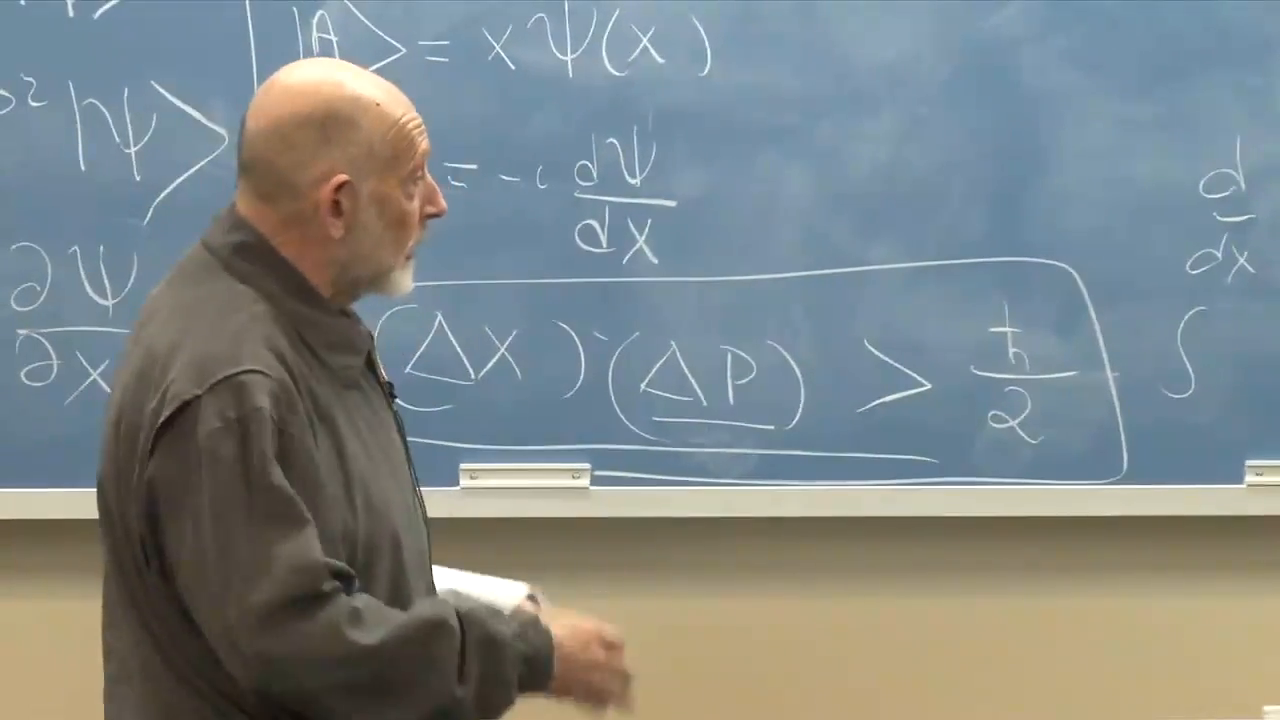
\includegraphics[width=0.88\textwidth]{lecture_10_figure_05.png}
\caption{Phép tích phân từng phần biến biểu thức bề ngoài mang dấu âm của \(\expect{P^2}\) thành một chuẩn dương tường minh.}
\lectureframe{00:27:35}
\end{figure}

\begin{classroomqa}
\audiencequestion{Có thể dời giá trị trung bình của cả vị trí lẫn xung lượng về không cùng một lúc không?}
\lecturerresponse{Có. Tịnh tiến đối số của hàm sóng làm dịch chuyển \(\expect{X}\), còn nhân nó với một pha sóng phẳng làm dịch chuyển \(\expect{P}\). Các phép biến đổi này thay đổi các giá trị trung bình mà không làm đổi các phương sai tương ứng, nên trong chứng minh có thể dùng cả hai biến đã được lấy tâm.}
\end{classroomqa}

\section{Cận bất định}

Công cụ toán học cần thiết là bất đẳng thức Cauchy--Schwarz. Bài giảng tiếp cận nó qua hình học vectơ sơ cấp: tích vô hướng của hai vectơ bằng độ dài của chúng nhân với cosin của góc giữa chúng, nên độ lớn của nó không thể vượt quá tích các độ dài ấy. Trong ký hiệu không gian Hilbert,
\begin{equation}
\braket{A}{A}\braket{B}{B}
\geq
\left|\braket{A}{B}\right|^2.
\label{eq:l10-cauchy-schwarz}
\end{equation}
Nó đúng trong các không gian vectơ thực hoặc phức với mọi số chiều.

\begin{figure}[htbp]
\centering
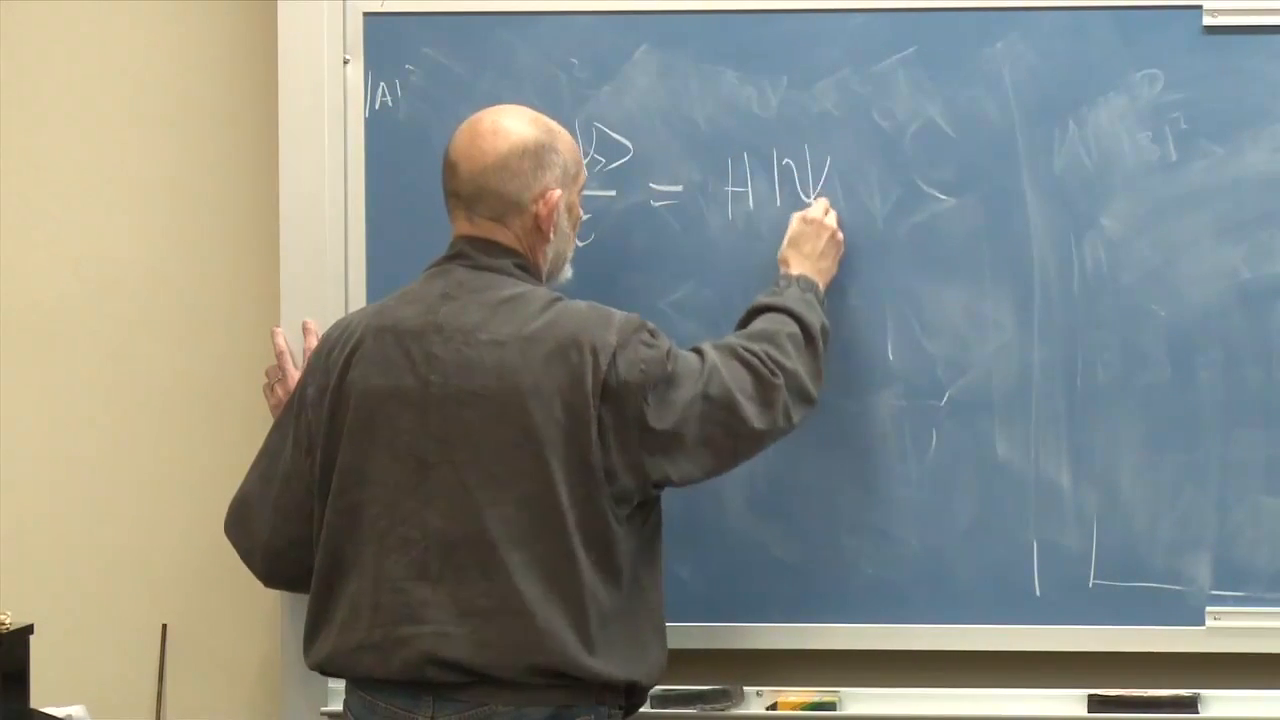
\includegraphics[width=0.88\textwidth]{lecture_10_figure_06.png}
\caption{Bất đẳng thức hình học của vectơ được viết lại thành cận Cauchy--Schwarz trong không gian Hilbert dùng trong chứng minh.}
\lectureframe{00:35:35}
\end{figure}

\begin{classroomqa}
\audiencequestion{Bất đẳng thức này phải là nghiêm ngặt, hay dấu bằng cũng có thể xảy ra?}
\lecturerresponse{Đó là một quan hệ lớn hơn hoặc bằng. Dấu bằng xảy ra khi hai vectơ trong không gian Hilbert phụ thuộc tuyến tính. Điều kiện đẳng thức ấy về sau xác định các gói sóng có độ bất định tối thiểu.}
\end{classroomqa}

Hãy lấy tâm cả hai biến và trước hết đi theo chứng minh giản lược trên bảng, trong đó giả sử \(\psi(x)\) là thực. Định nghĩa
\begin{equation}
\ket{A}=X\ket{\psi},
\qquad
\ket{B}=P\ket{\psi}.
\label{eq:l10-auxiliary-vectors}
\end{equation}
Bình phương chuẩn của chúng chính là các phương sai:
\begin{equation}
\braket{A}{A}=(\Delta x)^2,
\qquad
\braket{B}{B}=(\Delta p)^2.
\end{equation}

\begin{figure}[htbp]
\centering
\includegraphics[width=0.88\textwidth]{lecture_10_figure_07.png}
\caption{Các vectơ phụ trợ \(X\ket{\psi}\) và \(P\ket{\psi}\) biến hai phương sai thành các chuẩn trong không gian Hilbert.}
\lectureframe{00:44:40}
\end{figure}

Tích vô hướng còn lại là
\begin{align}
\braket{A}{B}
&=
\int_{-\infty}^{\infty}
dx\,
x\psi(x)
\left(-i\hbar\frac{d\psi}{dx}\right).
\end{align}
Chỉ trị tuyệt đối của nó mới đi vào. Vì \(\psi\) là thực,
\begin{equation}
\psi\frac{d\psi}{dx}
=
\frac{1}{2}\frac{d}{dx}\psi^2.
\end{equation}
Do đó,
\begin{align}
\left|\braket{A}{B}\right|
&=
\frac{\hbar}{2}
\left|
\int_{-\infty}^{\infty}
dx\,
x\frac{d}{dx}\psi^2
\right| \notag\\
&=
\frac{\hbar}{2}
\left|
-\int_{-\infty}^{\infty}
dx\,\psi^2
\right|
=
\frac{\hbar}{2},
\label{eq:l10-inner-product-half-hbar}
\end{align}
trong đó phép tích phân từng phần chuyển đạo hàm khỏi \(\psi^2\), \(d x/dx=1\), số hạng biên triệt tiêu, và điều kiện chuẩn hóa cho đẳng thức cuối cùng.

Thế Phương trình~\eqref{eq:l10-inner-product-half-hbar} vào bất đẳng thức Cauchy--Schwarz:
\begin{equation}
(\Delta x)^2(\Delta p)^2
\geq
\frac{\hbar^2}{4}.
\end{equation}
Lấy căn bậc hai dương cho ta
\begin{equation}
\boxed{
\Delta x\,\Delta p
\geq
\frac{\hbar}{2}
}.
\label{eq:l10-uncertainty-principle}
\end{equation}

\begin{figure}[htbp]
\centering
\includegraphics[width=0.88\textwidth]{lecture_10_figure_08.png}
\caption{Bước tích phân từng phần và phép chuẩn hóa cho ra cận bất định vị trí–xung lượng chặt.}
\lectureframe{00:50:55}
\end{figure}

Việc hạn chế \(\psi\) là thực chỉ là một thuận tiện trên bảng, không phải một hạn chế của định lý. Với một trạng thái phức tổng quát, lấy
\begin{equation}
\ket{A}=(X-\expect{X})\ket{\psi},
\qquad
\ket{B}=(P-\expect{P})\ket{\psi}.
\end{equation}
Giao hoán tử cố định phần ảo của tích vô hướng giữa chúng:
\begin{equation}
\operatorname{Im}\braket{A}{B}
=
\frac{1}{2i}\expect{[X,P]}
=
\frac{\hbar}{2}.
\end{equation}
Vì \(|\braket{A}{B}|\) ít nhất cũng lớn bằng độ lớn của phần ảo của nó, nên cùng một cận lại suy ra.

\begin{classroomqa}
\audiencequestion{Điều gì chính xác đã xảy ra với số hạng biên trong các lần tích phân từng phần lặp đi lặp lại?}
\lecturerresponse{Đối với các gói khả chuẩn hóa được xét ở đây, các tích xuất hiện tại \(+\infty\) và \(-\infty\) đều triệt tiêu. Trên một khoảng hữu hạn tuần hoàn, các số hạng ở hai đầu mút triệt tiêu lẫn nhau. Miền xác định của các toán tử phải được chọn sao cho các phát biểu này đúng; nếu không thì thao tác hình thức đó không được biện minh.}
\end{classroomqa}

\begin{classroomqa}
\audiencequestion{Dấu bằng có đạt được về mặt vật lý hay không, hay cận dưới chỉ là một ước lượng?}
\lecturerresponse{Có thể đạt được. Dấu bằng trong bất đẳng thức Cauchy--Schwarz đòi hỏi hai vectơ phụ trợ phải tỉ lệ với nhau. Giải điều kiện đó cho ra các gói Gauss, tức các trạng thái bất định tối thiểu sẽ được phát triển tiếp theo.}
\end{classroomqa}

\section{Các cặp liên hợp Fourier khác}

Quan hệ bất định giữa thời gian và năng lượng giống với quan hệ giữa vị trí và xung lượng. Tuy nhiên, nó đòi hỏi sự cẩn trọng hơn, vì ở đây thời gian thường là một tham số tiến hóa, không phải một đại lượng quan sát được biểu diễn bởi một toán tử tự liên hợp phổ quát. Hãy khai triển một trạng thái theo các vectơ riêng năng lượng:
\begin{equation}
\ket{\psi(t)}
=
\int dE\,
\phi(E)e^{-iEt/\hbar}\ket{E}.
\label{eq:l10-time-energy-fourier}
\end{equation}
Các biên độ năng lượng và sự biến thiên theo thời gian liên hệ với nhau theo Fourier. Một phân bố năng lượng hẹp biến thiên chậm và không thể tạo ra một xung được định thời sắc nét; một phân bố năng lượng rộng có thể tạo ra một đường bao thời gian đến ngắn.

\begin{figure}[htbp]
\centering
\includegraphics[width=0.88\textwidth]{lecture_10_figure_09.png}
\caption{Sự phụ thuộc thời gian được ghép từ các trạng thái riêng năng lượng với các pha \(e^{-iEt/\hbar}\), tạo nên cơ sở Fourier của quan hệ thời gian–năng lượng.}
\lectureframe{00:53:40}
\end{figure}

\begin{classroomqa}
\audiencequestion{Cùng một chứng minh ấy có áp dụng trực tiếp cho thời gian và năng lượng không?}
\lecturerresponse{Trực giác về độ rộng nghịch đảo thì có, và một gói sóng đi qua cho một ví dụ hữu ích: một khoảng thời gian đến ngắn đòi hỏi một phân bố năng lượng rộng. Phát biểu ở mức toán tử thì tinh tế hơn, vì trong cách xây dựng này thời gian không đi vào đúng theo cách \(X\) đi vào.}
\end{classroomqa}

Góc và mômen động lượng tạo thành một cặp liên hợp khác cho chuyển động quay. Cục bộ, quan hệ Fourier của chúng giống như vị trí và động lượng. Trên toàn cục, tính tuần hoàn của góc đòi hỏi phải cẩn trọng thêm, nên ở đây nhận xét này là một phép tương tự hơn là một định lý đầy đủ.

\begin{classroomqa}
\audiencequestion{Vị trí-động lượng, thời gian-năng lượng và góc-mômen động lượng có phải là những ví dụ biệt lập không?}
\lecturerresponse{Không. Các biến liên hợp chính tắc lặp đi lặp lại như những cặp Fourier. Chi tiết về miền xác định và tính tuần hoàn thì khác nhau, nhưng sự định xứ tương hỗ là cấu trúc chung.}
\end{classroomqa}

\section{Phương trình Schr\"odinger trong không gian vị trí}

Bây giờ ta quay lại động lực học. Định luật ở dạng trừu tượng là
\begin{equation}
i\hbar\frac{d}{dt}\ket{\psi(t)}
=
H\ket{\psi(t)}.
\label{eq:l10-abstract-schrodinger}
\end{equation}
Đối với một hạt khối lượng \(m\) trong một thế \(V(X)\), ta lấy
\begin{equation}
H=\frac{P^2}{2m}+V(X).
\label{eq:l10-particle-hamiltonian}
\end{equation}
Điều này đưa vào dạng động năng cộng thế năng của cơ học cổ điển, rồi kiểm tra xem sự tiến hóa lượng tử của nó có tái tạo chuyển động cổ điển trong chế độ thích hợp hay không.

\begin{figure}[htbp]
\centering
\includegraphics[width=0.88\textwidth]{lecture_10_figure_10.png}
\caption{Hamiltonian tác dụng lên vectơ trạng thái trừu tượng trong phương trình Schr\"odinger phụ thuộc thời gian.}
\lectureframe{00:59:05}
\end{figure}

Trong biểu diễn vị trí, \(P^2\) trở thành một đạo hàm bậc hai. Một hàm của \(X\) tác dụng bằng phép nhân:
\begin{equation}
\bigl(V(X)\psi\bigr)(x)=V(x)\psi(x).
\end{equation}
Do đó,
\begin{equation}
i\hbar\frac{\partial\psi(x,t)}{\partial t}
=
\left[
-\frac{\hbar^2}{2m}\frac{\partial^2}{\partial x^2}
+V(x)
\right]\psi(x,t).
\label{eq:l10-position-schrodinger}
\end{equation}

\begin{figure}[htbp]
\centering
\includegraphics[width=0.88\textwidth]{lecture_10_figure_11.png}
\caption{Hamiltonian của hạt trở thành phần động năng dạng đạo hàm bậc hai cộng với phép nhân bởi \(V(x)\).}
\lectureframe{01:03:05}
\end{figure}

\begin{classroomqa}
\audiencequestion{Theo nghĩa nào thì hàm thông thường \(V(x)\) là một toán tử?}
\lecturerresponse{Một khi đã chọn cơ sở vị trí, \(X\) tác dụng bằng cách nhân với \(x\). Vì thế một hàm đủ chính quy \(V(X)\) tác dụng bằng cách nhân với số tương ứng \(V(x)\) tại mỗi điểm. Tính hữu ích của nó được kiểm nghiệm bởi động lực học theo sau.}
\end{classroomqa}

Để tính các giá trị kỳ vọng, giải Phương trình~\eqref{eq:l10-position-schrodinger} theo hai đạo hàm theo thời gian:
\begin{align}
\dot{\psi}
&=
\frac{i\hbar}{2m}\psi''
-\frac{i}{\hbar}V\psi,
\label{eq:l10-psi-dot}\\
\dot{\psi}^{\,*}
&=
-\frac{i\hbar}{2m}\psi^{*\,\prime\prime}
+\frac{i}{\hbar}V\psi^*.
\label{eq:l10-psi-star-dot}
\end{align}
Dòng thứ hai chỉ là liên hợp phức của dòng thứ nhất, nhưng viết cả hai làm cho các sự triệt tiêu trở nên rõ ràng.

\section{Chuyển động của tâm gói sóng}

Tâm của phân bố vị trí là
\begin{equation}
\expect{X}
=
\int_{-\infty}^{\infty}
dx\,\psi^*(x,t)\,x\,\psi(x,t).
\end{equation}
Lấy đạo hàm theo thời gian:
\begin{equation}
\frac{d}{dt}\expect{X}
=
\int dx\,
\left(
\dot{\psi}^{\,*}x\psi
+
\psi^*x\dot{\psi}
\right).
\label{eq:l10-x-expectation-derivative}
\end{equation}
Hai hạng là liên hợp phức của nhau. Khi thay các Phương trình~\eqref{eq:l10-psi-dot} và \eqref{eq:l10-psi-star-dot} vào, các hạng thế triệt tiêu vì \(V(x)\) là thực. Lấy tích phân từng phần các hạng động năng còn lại ta được
\begin{align}
\frac{d}{dt}\expect{X}
&=
\frac{1}{m}
\int dx\,
\psi^*
\left(-i\hbar\frac{\partial}{\partial x}\right)
\psi \notag\\
&=
\frac{\expect{P}}{m}.
\label{eq:l10-ehrenfest-x}
\end{align}

\begin{figure}[htbp]
\centering
\includegraphics[width=0.88\textwidth]{lecture_10_figure_12.png}
\caption{Đạo hàm của tâm gói sóng rút gọn thành giá trị kỳ vọng của động lượng chia cho khối lượng.}
\lectureframe{01:15:40}
\end{figure}

Hệ thức này là chính xác. Không có phép gần đúng gói hẹp nào đi vào đại số đó.

\begin{classroomqa}
\audiencequestion{Trong phép suy dẫn này, giả thiết rằng gói sóng là một đỉnh hẹp đơn lẻ đã được dùng ở đâu?}
\lecturerresponse{Không ở đâu cả. Đồng nhất thức \(d\expect{X}/dt=\expect{P}/m\) đúng với mọi trạng thái trong miền xác định của Hamiltonian này. Sự định xứ chỉ quan trọng khi ta diễn giải \(\expect{X}\) như quỹ đạo của một hạt cổ điển.}
\end{classroomqa}

Nửa còn lại của cơ học liên quan đến động lượng:
\begin{equation}
\expect{P}
=
\int dx\,
\psi^*
\left(-i\hbar\frac{\partial}{\partial x}\right)
\psi.
\end{equation}
Lấy đạo hàm của cả hai thừa số phụ thuộc thời gian:
\begin{equation}
\frac{d}{dt}\expect{P}
=
-i\hbar
\int dx\,
\left(
\dot{\psi}^{\,*}\psi'
+
\psi^*\frac{\partial\dot{\psi}}{\partial x}
\right).
\label{eq:l10-p-expectation-start}
\end{equation}
Sau khi lấy tích phân từng phần một hạng, thay vào hai phương trình Schr\"odinger. Các đóng góp động năng triệt tiêu. Các hạng thế gộp lại thành
\begin{equation}
\int dx\,
V(x)
\left(
\psi\frac{\partial\psi^*}{\partial x}
+
\psi^*\frac{\partial\psi}{\partial x}
\right)
=
\int dx\,
V(x)\frac{\partial}{\partial x}|\psi|^2.
\end{equation}
Một phép tích phân từng phần cuối cùng chuyển đạo hàm sang thế:
\begin{align}
\frac{d}{dt}\expect{P}
&=
-\int dx\,|\psi(x,t)|^2\frac{dV}{dx} \notag\\
&=
-\expect{V'(X)}
\\
&=
\expect{F(X)},\\
F(x)&=-V'(x).
\label{eq:l10-ehrenfest-p}
\end{align}

\begin{figure}[htbp]
\centering
\includegraphics[width=0.88\textwidth]{lecture_10_figure_13.png}
\caption{Các hạng thế gộp thành một đạo hàm toàn phần, cho \(d\expect{P}/dt=-\expect{V'(X)}\).}
\lectureframe{01:30:45}
\end{figure}

Các Phương trình~\eqref{eq:l10-ehrenfest-x} và \eqref{eq:l10-ehrenfest-p} là định lý Ehrenfest cho Hamiltonian này. Chúng là các đồng nhất thức lượng tử chính xác, nhưng các phương trình chính xác cho giá trị kỳ vọng vẫn chưa phải là một quỹ đạo cổ điển.

\section{Nơi phép gần đúng cổ điển xuất hiện}

Cơ học cổ điển cho một điểm ở tâm gói sóng sẽ đòi hỏi
\begin{equation}
\frac{d}{dt}\expect{P}
\approx
F\!\left(\expect{X}\right).
\label{eq:l10-classical-center-force}
\end{equation}
Thay vào đó, cơ học lượng tử cho
\begin{equation}
\frac{d}{dt}\expect{P}
=
\expect{F(X)}.
\end{equation}
Nói chung,
\begin{equation}
\expect{F(X)}
\neq
F\!\left(\expect{X}\right).
\label{eq:l10-force-nonlinearity}
\end{equation}

\begin{classroomqa}
\audiencequestion{Nếu cả hai phương trình Ehrenfest đều chính xác, tại sao chúng vẫn chưa chứng minh rằng mọi trạng thái lượng tử đều tuân theo định luật Newton?}
\lecturerresponse{Định luật Newton cho tâm gói sóng cần lực được tính tại tâm. Phương trình lượng tử chính xác lại chứa giá trị trung bình của lực trên toàn bộ phân bố xác suất. Hai đại lượng đó trùng nhau đối với một gói hẹp trong một trường lực biến thiên chậm, nhưng không trùng nhau đối với một trạng thái tùy ý hay một lực phi tuyến.}
\end{classroomqa}

Phản ví dụ trong bài giảng làm cho sự phân biệt ấy trở nên không thể nhầm lẫn. Hãy lấy \(F(x)=x^2\) và chọn một trạng thái chuẩn hóa có hai đỉnh hẹp bằng nhau, tâm gần \(+a\) và \(-a\). Đối xứng cho
\begin{equation}
\expect{X}=0,
\qquad
F\!\left(\expect{X}\right)=0,
\end{equation}
trong khi
\begin{equation}
\expect{F(X)}
=
\expect{X^2}
\approx
a^2>0.
\end{equation}

\begin{figure}[htbp]
\centering
\includegraphics[width=0.88\textwidth]{lecture_10_figure_14.png}
\caption{Đối với một gói hai đỉnh đối xứng và \(F(x)=x^2\), lực tại giá trị trung bình triệt tiêu còn lực trung bình thì không.}
\lectureframe{01:33:35}
\end{figure}

Đối với một gói hẹp đơn lẻ có tâm tại \(\bar{x}=\expect{X}\), khai triển lực:
\begin{equation}
F(X)
=
F(\bar{x})
+
F'(\bar{x})(X-\bar{x})
+
\frac{1}{2}F''(\bar{x})(X-\bar{x})^2
+\cdots.
\end{equation}
Lấy giá trị kỳ vọng làm mất hạng tuyến tính:
\begin{equation}
\expect{F(X)}
=
F(\bar{x})
+
\frac{1}{2}F''(\bar{x})(\Delta x)^2
+\cdots.
\end{equation}
Phép gần đúng cổ điển đáng tin cậy khi gói sóng vẫn hẹp so với thang độ dài mà trên đó lực thay đổi đáng kể.

Các đặc trưng sắc nhọn có thể tách và tán xạ một gói sóng. Một thế rộng và trơn có xu hướng dẫn hướng một gói đủ định xứ mà không phá hủy dạng một đỉnh của nó; một vật cản dạng điểm, lõi nguyên tử, hay cấu trúc ở thang độ dài của bước sóng có thể tạo ra các thành phần phản xạ và nhiễu xạ.

\begin{figure}[htbp]
\centering
\includegraphics[width=0.88\textwidth]{lecture_10_figure_15.png}
\caption{Cấu trúc của thế ở một thang ngắn hơn bề rộng gói sóng hoặc bước sóng liên quan có thể bẻ một gói kết hợp thành các thành phần tán xạ.}
\lectureframe{01:37:25}
\end{figure}

\begin{classroomqa}
\audiencequestion{Điều gì khiến một thế trở nên xấu đối với một gói cổ điển?}
\lecturerresponse{Vấn đề là thang độ dài, không phải phẩm chất đạo đức. Những đặc trưng sắc hơn nhiều so với gói sóng hoặc có kích thước so sánh được với bước sóng của nó làm lộ ra bản chất sóng và sinh ra tán xạ. Nếu thế biến thiên chậm trên toàn gói sóng, lực gần như hằng trên miền đỡ của nó và tâm tuân theo phương trình cổ điển.}
\end{classroomqa}

Khối lượng cũng quan trọng. Đối với một gói gần đạt bất định tối thiểu,
\begin{equation}
\Delta x\,\Delta v
\sim
\frac{\hbar}{2m}.
\end{equation}
Khối lượng lớn cho phép đồng thời một bề rộng không gian nhỏ và một độ trải vận tốc vừa phải. Vì thế các vật nặng có thể vẫn được định xứ sắc nét khi đi qua các thế vĩ mô. Các hạt nhẹ dễ bị dàn trải hoặc nhiễu xạ hơn bởi cấu trúc vi mô. Đây là một lập luận về tỉ lệ, không phải khẳng định rằng chỉ riêng khối lượng quyết định chuyển động có cổ điển hay không.

\begin{classroomqa}
\audiencequestion{Theo nghĩa này, có khi nào electron đủ lớn để hành xử xấp xỉ cổ điển không?}
\lecturerresponse{Có, nếu trường ngoài biến thiên trơn trên thang của gói electron. Chẳng hạn, giữa hai bản tụ điện rộng, một gói sóng kết hợp có thể đi theo gia tốc cổ điển trong một khoảng thời gian hữu ích. Gần cấu trúc Coulomb sắc nhọn của hạt nhân, chính electron đó biểu hiện tán xạ rõ rệt.}
\end{classroomqa}

Thí nghiệm tán xạ năm 1911 của Rutherford đem lại bài học bổ sung. Các hạt alpha khi gặp phân bố điện tích cô đặc của một hạt nhân vàng đã bị tán xạ qua những góc lớn, cho thấy điện tích dương tập trung trong một vùng rất nhỏ. Rutherford mô tả một chùm hạt; cơ học lượng tử mô tả biên độ tới và các thành phần tán xạ của nó. Các thí nghiệm tán xạ electron và photon hiện đại khai thác cùng sự nhạy cảm với thang độ dài.

\begin{classroomqa}
\audiencequestion{Hành vi theo quan hệ giữa sóng và thang độ dài này có phải chỉ riêng các hạt vật chất mới có không?}
\lecturerresponse{Không. Sóng điện từ tuân theo quang học hình học khi chiết suất biến thiên chậm trên một bước sóng. Một cách tử nhiễu xạ có khoảng cách so sánh được với bước sóng sẽ làm sóng trải ra theo những hướng riêng biệt. Electron, hạt alpha, photon và các kích thích lượng tử khác đều chia sẻ mối liên hệ này giữa bước sóng và cấu trúc.}
\end{classroomqa}

Vì vậy, giới hạn cổ điển không phải là một định luật riêng biệt được dán chồng lên cơ học lượng tử. Các phương trình chính xác cho giá trị kỳ vọng đã chứa sẵn các quan hệ cổ điển. Các quỹ đạo cổ điển xuất hiện khi trạng thái vẫn được định xứ và Hamiltonian biến thiên đủ trơn để việc lấy trung bình lực trên thực tế tương đương với việc tính lực tại tâm gói sóng.